\begin{figure}[h]
    \centering
    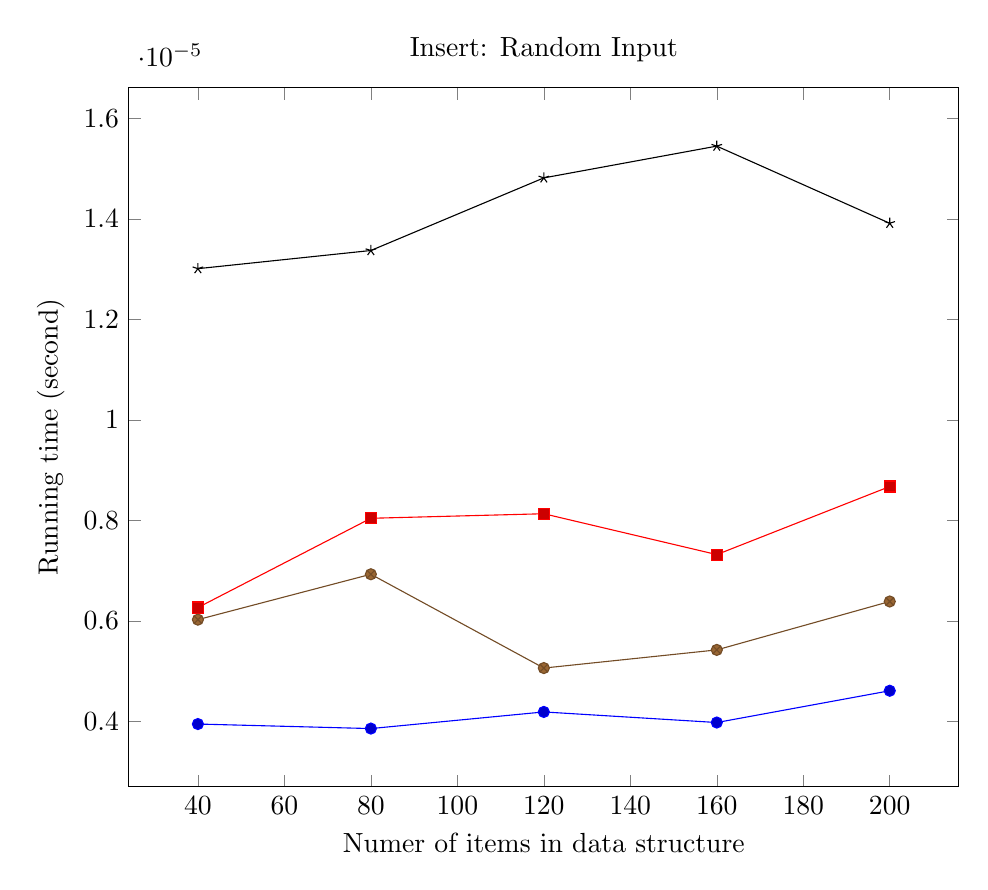
\begin{tikzpicture}
        \begin{axis}[
            xlabel={Numer of items in data structure},
            ylabel={Running time (second)},
            title={Insert: Random Input},
            width=\textwidth
        ]
		\addplot coordinates {
			(40, 3.945396911446408e-06)
			(80, 3.855044310421829e-06)
			(120, 4.186337180848987e-06)
			(160, 3.975514445121731e-06)
			(200, 4.607982652300724e-06)
		};
		\addplot coordinates {
			(40, 6.2644470044351254e-06)
			(80, 8.041381491270816e-06)
			(120, 8.131734092295395e-06)
			(160, 7.3185606830658554e-06)
			(200, 8.673849698448422e-06)
		};
		\addplot coordinates {
			(40, 6.023506735033934e-06)
			(80, 6.9270327452880535e-06)
			(120, 5.059745657429171e-06)
			(160, 5.421156061530263e-06)
			(200, 6.3849171391350264e-06)
		};
		\addplot coordinates {
			(40, 1.3010774547672632e-05)
			(80, 1.3372184951775112e-05)
			(120, 1.4817826568182257e-05)
			(160, 1.545029477536125e-05)
			(200, 1.3914300557928139e-05)
		};
        \legend{}
        \end{axis}
    \end{tikzpicture}
    \caption{Average of 0 operations, benchmarked every 0, starting at 0.}
\end{figure}